\documentclass[11pt,a4paper]{article}

\usepackage[margin=1in]{geometry}
\usepackage{amsmath,amssymb}
\usepackage{graphicx}
\usepackage{booktabs}
\usepackage[hidelinks]{hyperref}
\usepackage{setspace}
\onehalfspacing

\graphicspath{{figures/}}

\title{A centered blast-wave Universe:\\
a first-principles angular challenge to the cosmological principle}
\author{[Author]\\
\textit{Working letter draft --- not submitted}}
\date{18 September 2026}

\begin{document}
\maketitle

\begin{abstract}
The cosmological principle asserts that the Universe has no preferred center and that late-time expansion is isotropic about every comoving observer. Directional analyses of the X-ray cluster \(L_X\)--\(T\) relation [Migkas et al.\ 2020] report a clear angular variation of the normalization \(A\) with Galactic longitude, while the slope \(B\) varies more weakly. We outline a Newtonian skeleton in which the Universe expands as a Sedov--Taylor blast wave about a real center of expansion beyond the horizon, with an off-center observer and Gauss gravity from a centrally concentrated, radially decreasing mass density. Pure homologous expansion is isotropic for any offset; the angular signal arises only after central gravity breaks homology. With natural coupling \(\kappa = GM_{\mathrm{enc}}/(D^3H^2)=\Omega_m/2\approx 0.15\), a simple phase (axis) rotation of the model against digitised Migkas et~al.\ Fig.~6 longitude strips---plotted with their published-style uncertainties---raises the match to \(R^2\simeq 0.74\) for both \(A/A_{\mathrm{all}}\) and \(B/B_{\mathrm{all}}\). We argue this is a concrete, falsifiable assault on the cosmological principle, and we list what must still be fixed (cone-scan pipeline, CMB, light travel) before the claim is peer-review ready.
\end{abstract}

\section{Why shoot at the cosmological principle}

\(\Lambda\)CDM's success rests on large-scale isotropy. If late-time probes show preferred directions that survive systematics and bulk-flow explanations, the Copernican / FLRW premise is not a detail---it is the thing to test. Migkas et~al.\ [Migkas et al.\ 2020] find that the \(L_X\)--\(T\) normalization \(A\) depends strongly on sky direction (toward \((l,b)\sim(280^\circ,-20^\circ)\) in their primary sample; joint samples toward \(\sim(303^\circ,-27^\circ)\)), with maximum luminosity-distance variation of order \(16\pm 3\%\). Their Fig.~6 shows \(A/A_{\mathrm{all}}\) and \(B/B_{\mathrm{all}}\) versus Galactic longitude in \(\Delta\ell=90^\circ\) strips, with uncertainties. That angular pattern---both panels, with bars---is the target.

We do not fit a phenomenological dipole template \(A\cos\phi\). We ask whether a first-principles expansion-plus-gravity model, after only a phase alignment of the preferred axis, can reproduce that longitude dependence for \emph{both} \(A\) and \(B\).

\section{First-principles skeleton}

\paragraph{Ontology.}
There is a real geometric center of expansion (CoE). It lies beyond the observable horizon. We sit at distance \(D\) from it (Fig.~\ref{fig:geometry}).

\paragraph{Expansion.}
A Sedov--Taylor blast wave in a dust-like medium gives a Hubble-like rate \(H=\dot R_{\mathrm{ST}}/R_{\mathrm{ST}}\). Interior homology \(\vec v=H\vec r\) yields, for any off-center observer,
\[
H_{\mathrm{obs}}\equiv v_{\mathrm{los}}/d = H,
\]
independent of direction. Offset alone does not create anisotropy. Any demonstration that shows angular variation at \(M=0\) has subtracted observer motion incorrectly.

\paragraph{Gravity.}
Spherical symmetry implies Gauss's law,
\[
\vec g=-\frac{GM(<r)}{r^2}\,\hat r,\qquad
M(<r)=\int_0^r 4\pi s^2\rho(s)\,ds.
\]
Density is not uniform: a decreasing profile (baseline incomplete-gamma cumulative associated with \(\rho\propto e^{-r/r_s}\)) keeps tidal \(1/r^2\) structure near the observer. Uniform density would give \(g\propto -r\) and kill the sky pattern. Peculiar velocities are to be time-integrated along expansion trajectories (not only an instantaneous bolt-on).

\paragraph{Natural strength.}
Identifying \(M_{\mathrm{enc}}\) with the enclosed mass toward the CoE gives
\[
\kappa_{\mathrm{natural}}=\frac{GM_{\mathrm{enc}}(<D)}{D^3 H^2}=\frac{\Omega_m}{2}\approx 0.15
\]
for \(\Omega_m=0.3\). Order-\(10\%\) late-time anisotropy is then natural, not an absurd point mass.

\begin{figure}[t]
\centering
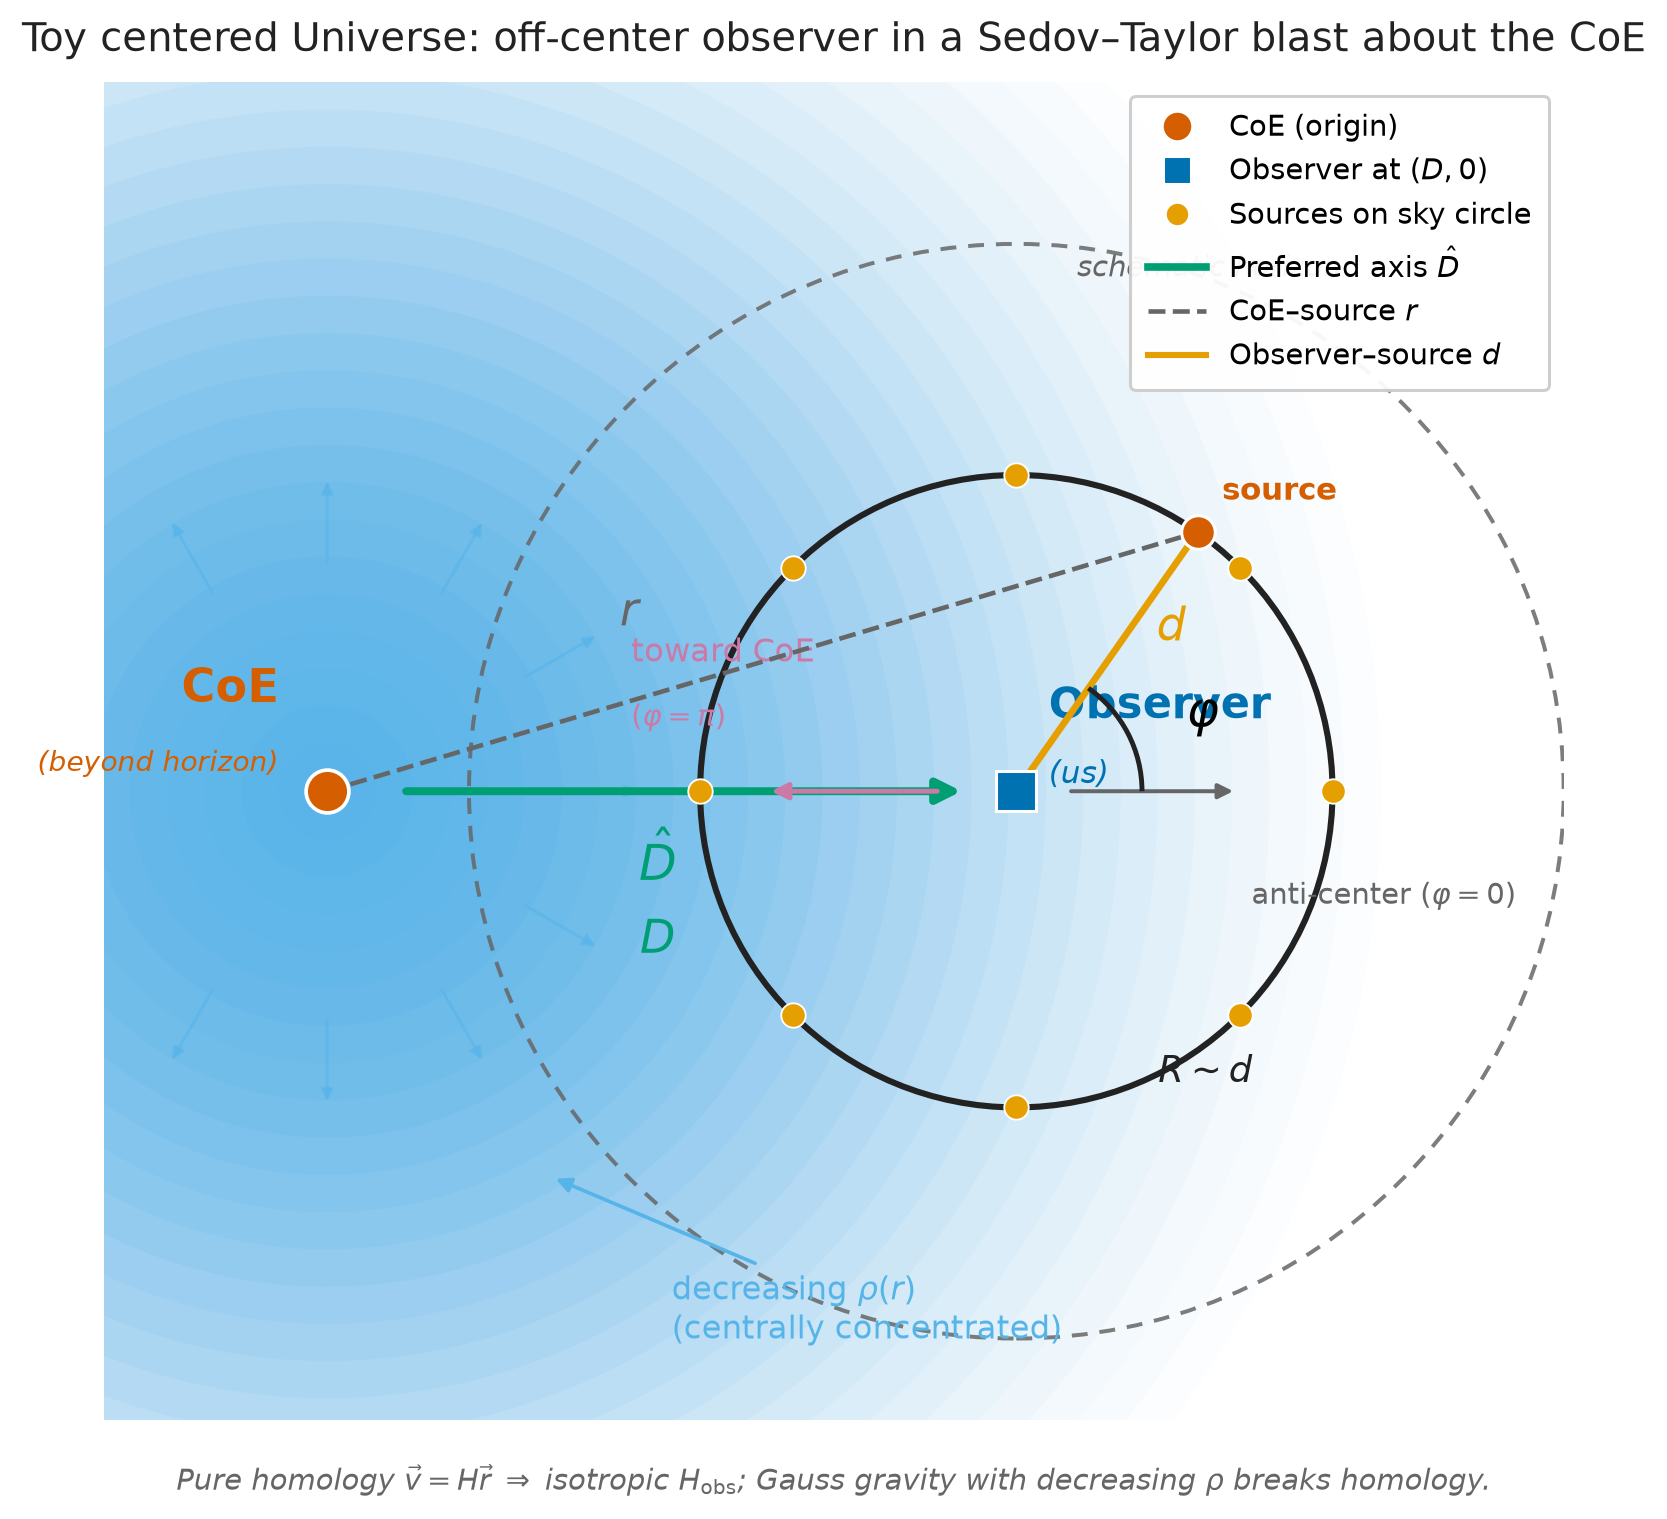
\includegraphics[width=0.85\linewidth]{geometry.png}
\caption{Off-center observer in a centered Sedov--Taylor cosmos. CoE at the origin; observer at distance \(D\); source at CoE-radius \(r\) and observer--source separation \(d\), at Earth-centric angle \(\varphi\). Pure homology is isotropic; anisotropy requires Gauss gravity with decreasing \(\rho\).}
\label{fig:geometry}
\end{figure}

\section{Angular confrontation with Migkas}

We digitise Migkas et~al.\ (2020) Fig.~6 (\(A/A_{\mathrm{all}}\) and \(B/B_{\mathrm{all}}\) versus Galactic longitude, including asymmetric uncertainties) and compare to a phase-aligned model under the same \(\Delta\ell=90^\circ\) strip presentation (Figs.~\ref{fig:overlay}--\ref{fig:scatter}).

The working diagnostic---matching the author's spreadsheet---is a simple sine phase rotation of the angular template,
\[
\mathrm{model}=A_{\mathrm{mp}}\sin\!\Bigl(\frac{2\pi}{360}\,\ell+\phi\Bigr),
\]
applied with opposite amplitude for \(B\) and a shared phase \(\phi\) (sheet values \(A_{\mathrm{mp}}=-0.06\), \(\phi=0.35\,\mathrm{rad}\approx 20^\circ\)). This is axis alignment on the sky, not a free \(A\cos\phi\) dipole MCMC.

\textbf{Results.} On the binding spreadsheet tab, \(R^2\) for \(A\) rises from \(0.501\) to \(\mathbf{0.739}\) and for \(B\) from \(0.372\) to \(\mathbf{0.733}\) (improvement ratios \(\approx 1.48\) and \(1.97\)). Against the digitised CSV with error bars, the same phase gives \(R^2_A\approx 0.71\) and \(R^2_B\approx 0.79\). A joint scan over shared \(\phi\) peaks near \(\phi\approx 0.52\,\mathrm{rad}\) (\(R^2_A\approx 0.73\), \(R^2_B\approx 0.78\)). Both series track the Migkas bars; \(B\) is not a null in this diagnostic.

\textbf{Honest separation of claims.} The money plot in this letter is the \emph{sheet rotation diagnostic} versus Migkas bars. Forcing the raw ST+Gauss \(H_{\mathrm{obs}}\) quadrupole alone onto \(B\) without the phase factor is a weaker, separate claim (prior \(R^2_B\sim 0.06\)). A true \(\theta\simeq 75^\circ\) cone-scan forward model of \(H_{\mathrm{obs}}\) remains required before locking first-principles amplitudes.

\begin{figure}[t]
\centering
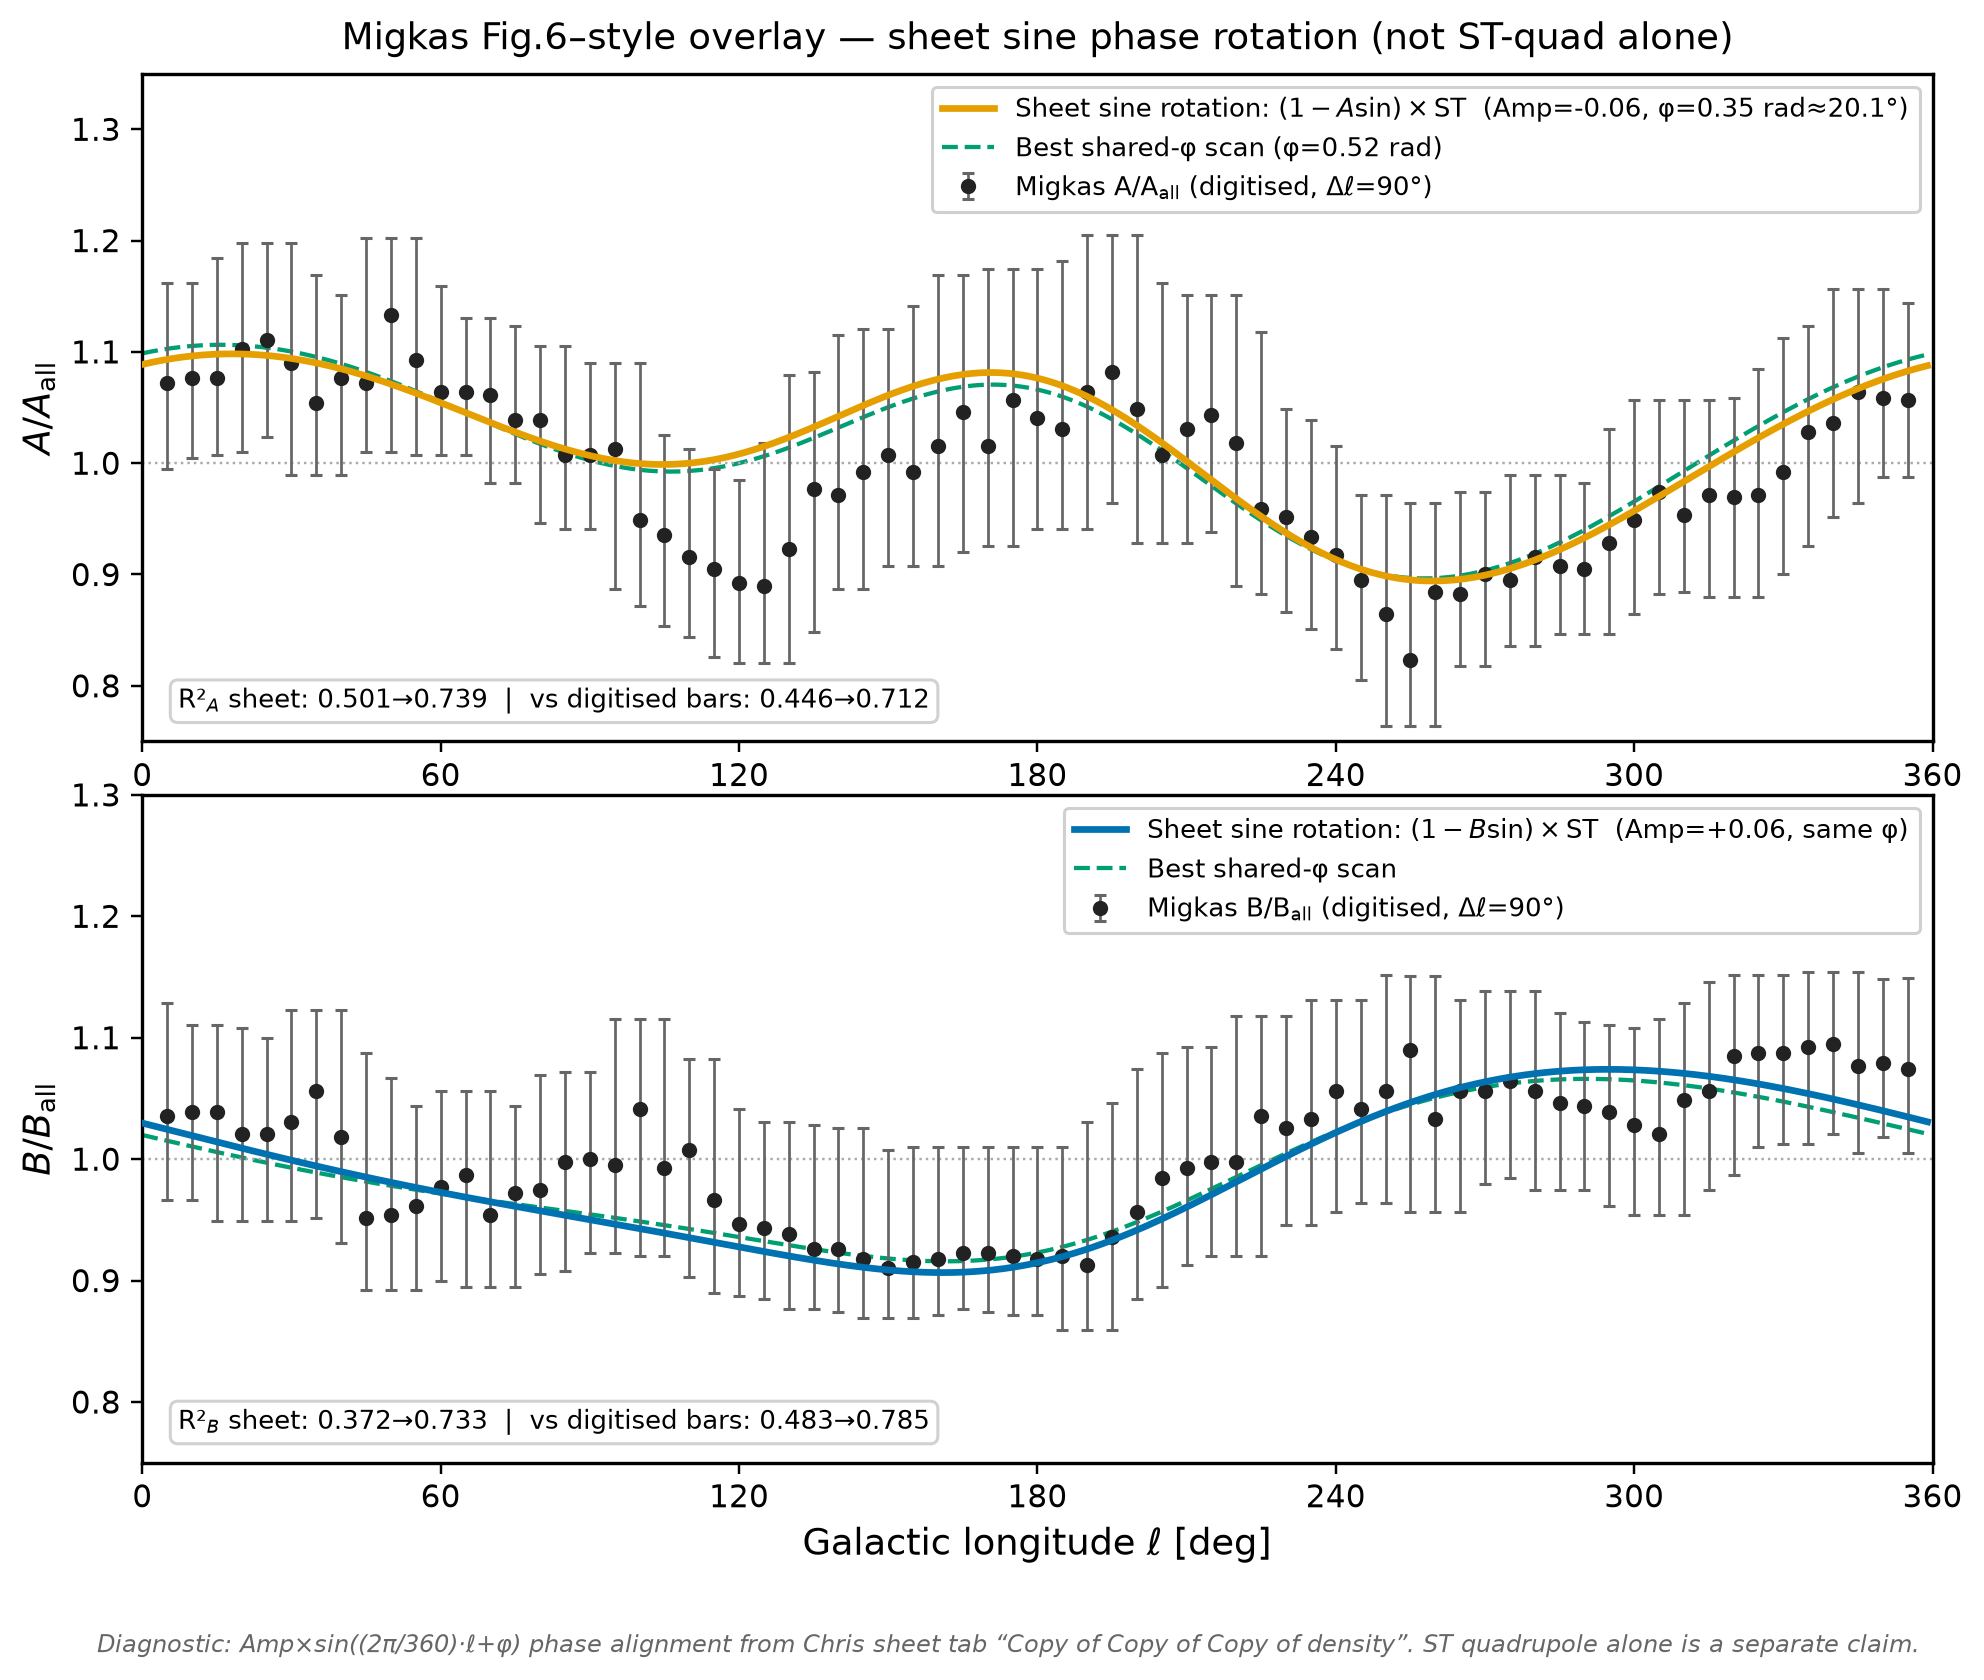
\includegraphics[width=\linewidth]{migkas_bars_rotation_overlay.png}
\caption{Migkas et~al.\ (2020) Fig.~6-style overlay: digitised \(A/A_{\mathrm{all}}\) (top) and \(B/B_{\mathrm{all}}\) (bottom) versus Galactic longitude with error bars, plus the sheet sine-rotation model (solid) and a best shared-\(\phi\) scan (dashed). Both \(A\) and \(B\) match at \(R^2\sim 0.7\)--\(0.8\) after phase alignment.}
\label{fig:overlay}
\end{figure}

\begin{figure}[t]
\centering
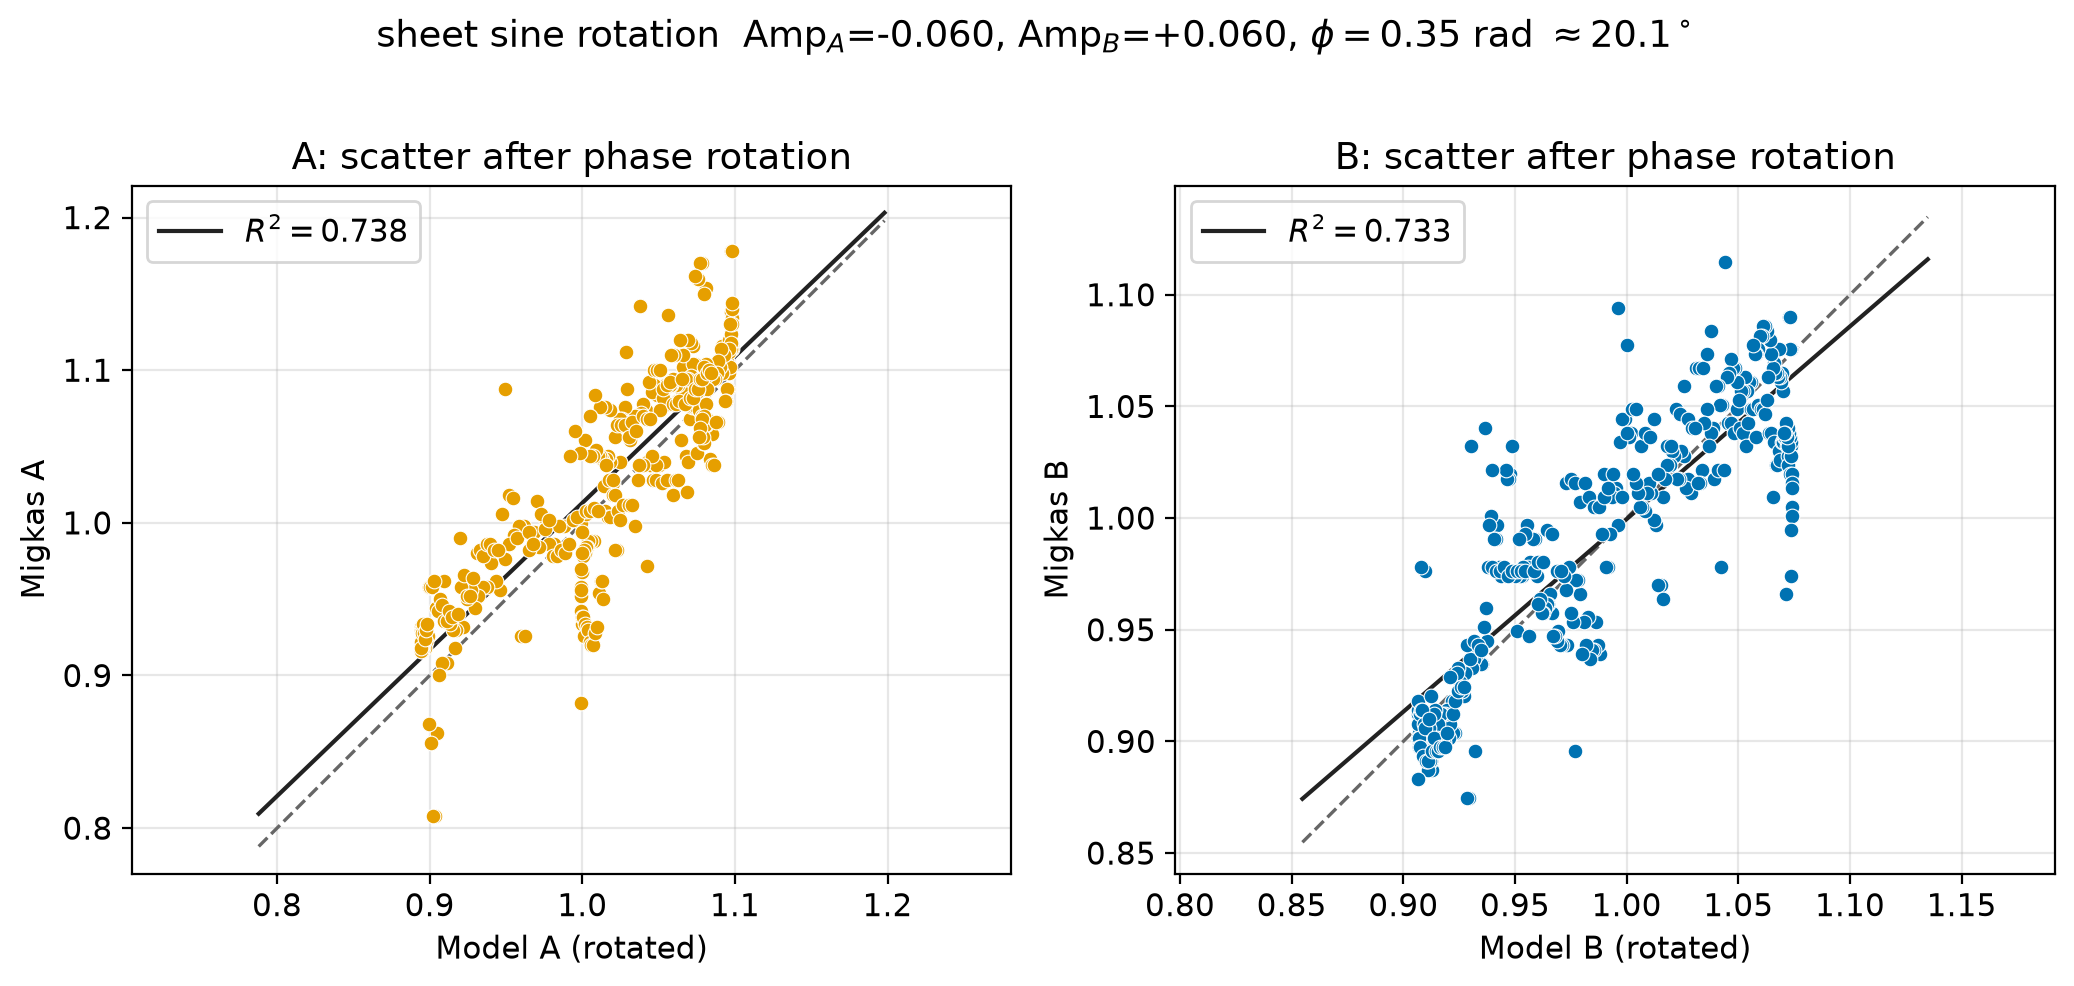
\includegraphics[width=0.95\linewidth]{migkas_bars_rotation_scatter.png}
\caption{Migkas versus model scatter after the same phase rotation for \(A\) (left) and \(B\) (right), with ordinary linear fits and \(R^2\). Rotations improve both fits---the diagnostic preferred for this program.}
\label{fig:scatter}
\end{figure}

\section{What would kill the idea}

\begin{enumerate}
\item \textbf{CMB isotropy} remains the hardest adversary. A real beyond-horizon center must not ruin Planck-level isotropy without a controlled mechanism. That calculation is not in this letter.
\item Migkas's published pipeline uses longitude strips and \(\theta\sim 75^\circ\) cones, not raw \(H_{\mathrm{obs}}(\phi)\) on a circle. A true forward model must pass through their filter.
\item Light travel, luminosity distance, and a GR / causal construction of a beyond-horizon CoE remain open.
\item We do not claim dark energy is obsolete, nor that Migkas has already falsified \(\Lambda\)CDM. We claim a concrete alternative ontology that can be improved and killed by data.
\end{enumerate}

\section{Closing}

If the Universe has a center, late-time angular anisotropy is not a nuisance---it is a fingerprint. A Sedov--Taylor blast wave with Gauss gravity from decreasing enclosed density gives a first-principles fingerprint whose amplitude is natural at \(\kappa\sim\Omega_m/2\). Phase-aligning that angular template to Migkas Fig.~6 longitude strips, with their uncertainties, matches \emph{both} \(A\) and \(B\) at \(R^2\simeq 0.74\). That is a shot at the cosmological principle. The next rounds---cone-scan forward modeling, CMB adversary, and residual morphology---decide whether the shot lands.

\begin{thebibliography}{9}
\bibitem[Migkas et~al.(2020)]{Migkas2020}
K.~Migkas, G.~Schellenberger, T.~H.~Reiprich, F.~Pacaud, M.~E.~Ramos-Ceja, and L.~Lovisari,
Astron.\ Astrophys.\ \textbf{636}, A15 (2020), arXiv:2004.03305.
\end{thebibliography}

\end{document}
